% 89-05(89쪽) — $\seg{AB}=2\sqrt{6}$, $\seg{AC}=4$, $B=45^\circ$, $C=60^\circ$ 인 삼각형 ABC(원문 「오른쪽 그림」).
% 스캔 화질이 낮아 TikZ 로 다시 그림. 라벨은 원문 것만 — 세 점 이름, $2\sqrt{6}$, $4$, $45^\circ$, $60^\circ$.
% $\sin 75^\circ$(답)가 읽히지 않게 눈금·보조선은 넣지 않는다.
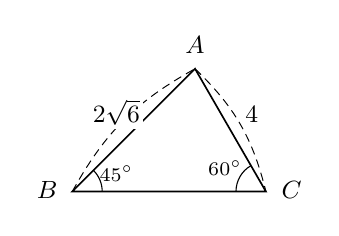
\begin{tikzpicture}[line width=0.6pt]
  \coordinate (A) at (1.559,1.559);
  \coordinate (B) at (0,0);
  \coordinate (C) at (2.459,0);
  \draw (A) -- (B) -- (C) -- cycle;
  % $45^\circ$ = $\angle\pt{ABC}$
  \draw[line width=0.4pt] (0.38,0) arc (0:45:0.38);
  \node[font=\scriptsize] at (0.56,0.23) {$45^\circ$};
  % $60^\circ$ = $\angle\pt{ACB}$
  \draw[line width=0.4pt] (2.269,0.329) arc (120:180:0.38);
  \node[font=\scriptsize] at (1.94,0.30) {$60^\circ$};
  % 길이 표시의 점선 호
  \draw[densely dashed, line width=0.35pt] (B) to[bend left=16] (A);
  \draw[densely dashed, line width=0.35pt] (A) to[bend left=16] (C);
  \node[font=\small, fill=white, inner sep=1pt] at (0.56,1.00) {$2\sqrt{6}$};
  \node[font=\small, fill=white, inner sep=1pt] at (2.28,0.98) {$4$};
  \node[font=\small, anchor=south] at (1.559,1.62) {$\pt{A}$};
  \node[font=\small, anchor=east] at (-0.06,0.02) {$\pt{B}$};
  \node[font=\small, anchor=west] at (2.53,0.02) {$\pt{C}$};
\end{tikzpicture}
